\section{Hiện thực hệ thống}

\subsection{Cấu trúc mã nguồn}
\subsubsection{Frontend}

\begin{figure}[H]
	\centering
	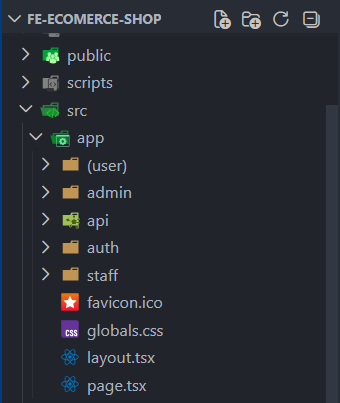
\includegraphics[width=0.8\textwidth]{Images/sourceCodeStructureImgs/frontend-1.png}
	\vspace{0.5cm}
	\caption{Cấu trúc mã nguồn frontend}
	\label{fig: Cấu trúc mã nguồn frontend}
\end{figure}

Trong đó: \\
Folder public: Chứa các tài nguyên tĩnh của website như hình ảnh, icon, font, file tải xuống và các tài nguyên được trình duyệt truy cập trực tiếp. \\

Folder scripts: Chứa các script hỗ trợ quá trình chạy dự án, thường dùng để cấu hình môi trường, tự động hóa lệnh hoặc xử lý các tác vụ dev. \\

Folder src: Chứa toàn bộ mã nguồn chính của frontend, bao gồm giao diện, logic gọi API, kiểu dữ liệu, hook và các tiện ích dùng chung. \\

Folder app: Chứa hệ thống route theo App Router của Next.js, là nơi định nghĩa các trang, layout, API route và các nhóm route của toàn bộ ứng dụng. \\

Folder (user): Chứa nhóm route dành cho người dùng thông thường, tách biệt với khu vực admin và staff để dễ quản lý giao diện và logic theo vai trò. \\

Folder admin: Chứa toàn bộ giao diện và trang quản trị hệ thống như dashboard, quản lý sản phẩm, danh mục, đơn hàng, người dùng và các tính năng vận hành. \\

Folder api: Chứa các API routes phía server của Next.js, thường được dùng làm lớp trung gian gọi backend hoặc xử lý request đặc thù. \\

Folder auth: Chứa các trang và luồng liên quan đến xác thực như đăng nhập, đăng ký, xử lý phiên đăng nhập hoặc các thao tác bảo mật. \\

Folder staff: Chứa các trang và chức năng dành cho nhân viên hệ thống, thường có phạm vi quyền hạn nhỏ hơn admin. \\

File favicon.ico: Là biểu tượng hiển thị trên tab trình duyệt, giúp nhận diện website nhanh hơn. \\

File globals.css: Chứa các style toàn cục áp dụng cho toàn bộ ứng dụng, bao gồm biến màu, reset CSS và cấu hình giao diện nền tảng. \\

File layout.tsx: Là layout gốc bao quanh toàn bộ ứng dụng, thường chứa cấu trúc HTML chung, provider và các thành phần dùng lại trên mọi trang. \\

File page.tsx: Là trang chủ mặc định của website, nơi hiển thị nội dung chính khi người dùng truy cập vào domain gốc. \\


\begin{figure}[H]
	\centering
	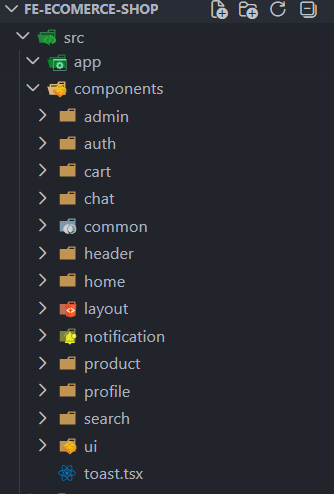
\includegraphics[width=0.8\textwidth]{Images/sourceCodeStructureImgs/frontend-2.png}
	\vspace{0.5cm}
	\caption{Cấu trúc mã nguồn frontend (Tiếp theo)}
	\label{fig: Cấu trúc mã nguồn frontend (Tiếp theo)}
\end{figure}

Trong đó: \\

Folder components: Chứa toàn bộ các component giao diện tái sử dụng trong dự án, được chia nhỏ theo từng nhóm chức năng để dễ bảo trì và mở rộng. \\

Folder admin: Chứa các component phục vụ riêng cho trang quản trị, như bảng dữ liệu, form quản lý, sidebar, modal và các khối UI của admin. \\

Folder auth: Chứa các component liên quan đến xác thực như form đăng nhập, đăng ký, xác nhận tài khoản và các màn hình bảo mật. \\

Folder cart: Chứa các component xử lý giỏ hàng và thanh toán, bao gồm danh sách sản phẩm trong giỏ, tổng tiền và nút thao tác mua hàng. \\

Folder chat: Chứa các component cho tính năng chat realtime giữa người dùng và hệ thống hoặc giữa các vai trò khác nhau. \\

Folder common: Chứa các component dùng chung như breadcrumb, pagination, empty state, modal, alert và các thành phần trung lập cho nhiều màn hình. \\

Folder header: Chứa các component của phần đầu trang như logo, menu điều hướng, tìm kiếm, tài khoản và các nút hành động chính. \\

Folder home: Chứa các component hiển thị trên trang chủ như banner, danh mục nổi bật, sản phẩm nổi bật và các block giới thiệu nội dung. \\

Folder layout: Chứa các component bố cục dùng chung như footer, sidebar, wrapper và những khung sườn giao diện của toàn trang. \\

Folder notification: Chứa các component hiển thị thông báo, toast hoặc danh sách thông báo cho người dùng. \\

Folder product: Chứa các component liên quan đến sản phẩm như card sản phẩm, bộ lọc, danh sách sản phẩm, chi tiết sản phẩm và các phần mở rộng. \\

Folder profile: Chứa các component cho trang hồ sơ người dùng, bao gồm thông tin cá nhân, đơn hàng, địa chỉ và các thiết lập tài khoản. \\

Folder search: Chứa các component phục vụ tìm kiếm sản phẩm, lọc kết quả và hiển thị dữ liệu theo từ khóa. \\

Folder ui: Chứa bộ component giao diện cơ bản, thường là các primitive UI như button, input, dialog, select, badge và các component nền tảng khác. \\

File toast.tsx: Chứa cấu hình hoặc component xử lý thông báo toast toàn cục trong ứng dụng. \\

\begin{figure}[H]
	\centering
	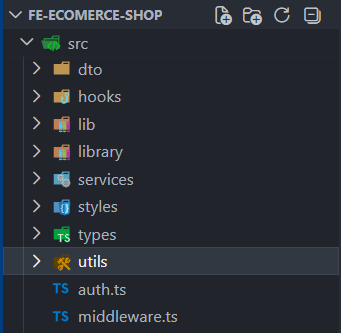
\includegraphics[width=0.8\textwidth]{Images/sourceCodeStructureImgs/frontend-3.png}
	\vspace{0.5cm}
	\caption{Cấu trúc mã nguồn frontend (Tiếp theo)}
	\label{fig: Cấu trúc mã nguồn frontend (Tiếp theo)}
\end{figure}

Trong đó: \\

Folder dto: Chứa các kiểu dữ liệu và interface TypeScript mô tả cấu trúc request/response của backend, giúp toàn bộ dự án dùng type an toàn. \\

Folder hooks: Chứa các custom hook React để tái sử dụng logic như kết nối socket, quản lý state đặc thù hoặc các hành vi phức tạp. \\

Folder lib: Chứa các hàm thư viện nội bộ, tiện ích kỹ thuật hoặc các cấu hình logic dùng chung cho toàn project. \\

Folder library: Chứa các lớp hoặc wrapper thư viện đặc thù của dự án, thường dùng để tích hợp hoặc chuẩn hóa cách sử dụng một số công cụ bên ngoài. \\

Folder services: Chứa tầng gọi API đến backend, mỗi file tương ứng với một nhóm nghiệp vụ như sản phẩm, đơn hàng, giỏ hàng, thanh toán, người dùng và thông báo. \\

Folder styles: Chứa các file style và theme toàn cục, bao gồm biến CSS, theme riêng cho từng khu vực như storefront và admin. \\

Folder types: Chứa các định nghĩa kiểu TypeScript bổ sung cho toàn dự án, ví dụ mở rộng kiểu của thư viện bên ngoài hoặc kiểu dữ liệu dùng chung. \\

Folder utils: Chứa các hàm tiện ích hỗ trợ như xử lý lỗi, wrapper gọi API, format dữ liệu và các logic nhỏ dùng lại ở nhiều nơi. \\

File auth.ts: Chứa cấu hình xác thực của dự án, liên quan đến session, provider đăng nhập và cách quản lý trạng thái đăng nhập. \\

File middleware.ts: Chứa middleware chạy trung gian trước khi vào route, thường dùng để kiểm tra quyền truy cập, điều hướng và bảo vệ trang. \\

\subsubsection{Backend}
\begin{figure}[H]
	\centering
	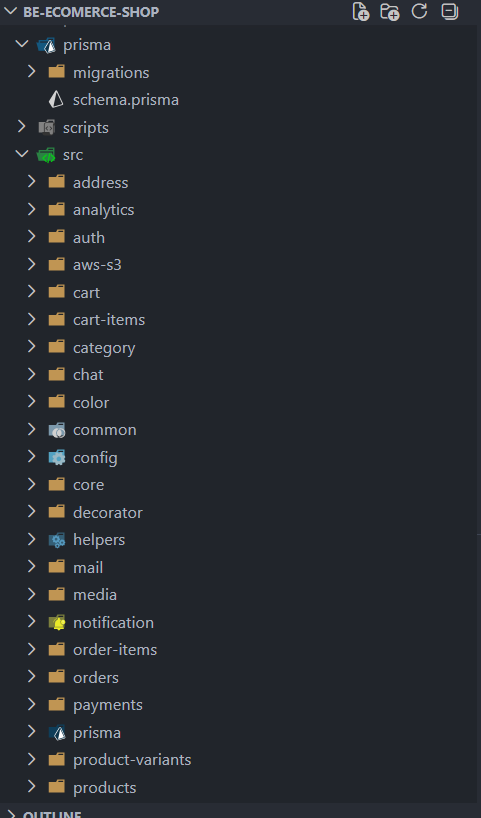
\includegraphics[width=0.8\textwidth]{Images/sourceCodeStructureImgs/backend-1.png}
	\vspace{0.5cm}
	\caption{Cấu trúc mã nguồn backend}
	\label{fig: Cấu trúc mã nguồn backend}
\end{figure}

Trong đó: \\

Folder prisma: Chứa tất cả các bản migration database của dự án. Và chứa file schema.prisma đây là file chứa toàn bộ model của dự án. Các model này sẽ được Prisma Orm dịch tự động thành các bảng của Postgres. \\

Trong folder src, các folder tiếp theo sẽ đảm nhiệm logic cho một số nhiệm vụ cụ thể như sau: \\

Folder address: Chịu trách nhiệm cho toàn bộ logic liên quan đến CURD địa chỉ của người dùng, order, shipment. \\

Folder analytics: Chịu trách nhiệm tổng hợp và phân tích dữ liệu kinh doanh như doanh số, số lượng đơn hàng đã bán, đã hủy, đã hoàn, phân tích thanh toán, tồn kho, khách hàng mới và khách hàng quay lại, cùng các thống kê phục vụ dashboard quản trị. \\

Folder auth: Xử lý xác thực và phân quyền người dùng, bao gồm đăng nhập, JWT, OAuth, các strategy và guard bảo vệ API. \\

Folder aws-s3: Chứa logic làm việc với AWS S3, chủ yếu phục vụ việc tải lên, lưu trữ và quản lý tệp tin trên cloud. \\

Folder cart: Quản lý giỏ hàng của người dùng, bao gồm các thao tác tạo, cập nhật, xóa và tính toán giỏ hàng. \\

Folder cart-items: Quản lý chi tiết từng sản phẩm nằm trong giỏ hàng. \\

Folder category: Quản lý danh mục sản phẩm, phục vụ phân loại và tổ chức sản phẩm trong hệ thống. \\

Folder chat: Chịu trách nhiệm cho chức năng chat realtime, bao gồm phòng chat, tin nhắn và kết nối WebSocket. \\

Folder color: Quản lý thuộc tính màu sắc của sản phẩm. \\

Folder common: Chứa các thành phần dùng chung cho toàn bộ dự án, đặc biệt là các cấu hình hoặc tài nguyên hỗ trợ Swagger/OpenAPI. \\

Folder config: Chứa các file cấu hình khởi tạo và tích hợp các dịch vụ nền như Bull queue và Mailer. \\

Folder core: Chứa các thành phần lõi ở mức toàn cục của hệ thống, ví dụ interceptor dùng để chuẩn hóa dữ liệu phản hồi. \\

Folder decorator: Chứa các custom decorator được tạo riêng để tái sử dụng trong nhiều module khác nhau. \\

Folder helpers: Chứa các hàm tiện ích, service hỗ trợ và các kiểu dữ liệu dùng chung cho nhiều phần của dự án. \\

Folder mail: Chịu trách nhiệm gửi email, quản lý template email và các logic liên quan đến mail trong hệ thống. \\

Folder media: Quản lý tệp media, bao gồm lưu trữ thông tin file và xử lý các tài nguyên đa phương tiện. \\

Folder notification: Xử lý hệ thống thông báo, bao gồm thông báo realtime và các logic phát sinh thông báo cho người dùng. \\

Folder order-items: Quản lý chi tiết sản phẩm trong từng đơn hàng. \\

Folder orders: Chịu trách nhiệm cho toàn bộ vòng đời của đơn hàng, từ khởi tạo, xử lý, xác nhận đến liên kết với thanh toán và giao hàng. \\

Folder payments: Xử lý thanh toán trực tuyến, tích hợp cổng thanh toán và theo dõi trạng thái thanh toán của đơn hàng. \\

Folder prisma: Chứa module kết nối Prisma, cung cấp PrismaService để toàn bộ hệ thống truy cập cơ sở dữ liệu một cách thống nhất. \\

Folder product-variants: Quản lý các biến thể sản phẩm như kích thước, màu sắc, tồn kho và thông tin biến thể đi kèm. \\

Folder products: Chịu trách nhiệm cho CRUD sản phẩm, danh sách sản phẩm, lọc tìm kiếm và thông tin hiển thị của sản phẩm. \\

\begin{figure}[H]
	\centering
	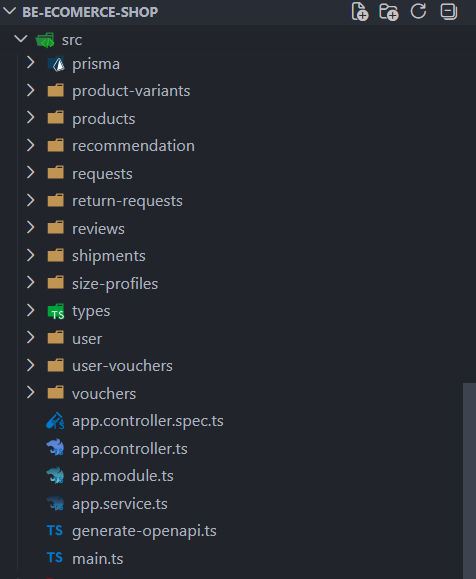
\includegraphics[width=0.8\textwidth]{Images/sourceCodeStructureImgs/backend-2.png}
	\vspace{0.5cm}
	\caption{Cấu trúc mã nguồn backend (Tiếp theo)}
	\label{fig: Cấu trúc mã nguồn backend (Tiếp theo)}
\end{figure}

Folder recommendation: Chứa logic gợi ý sản phẩm cho người dùng và các tác vụ liên quan đến tính toán đề xuất. \\

Folder requests: Quản lý các yêu cầu do người dùng gửi lên hệ thống. \\

Folder return-requests: Xử lý yêu cầu trả hàng, hoàn hàng hoặc đổi trả của khách hàng. \\

Folder reviews: Quản lý đánh giá sản phẩm, bình luận và các media đi kèm với bài đánh giá. \\

Folder shipments: Chịu trách nhiệm cho logic vận chuyển, tạo đơn giao hàng, tính phí ship và tích hợp đơn vị vận chuyển. \\

Folder size-profiles: Quản lý thông tin size profile để hỗ trợ sản phẩm có nhiều bảng size khác nhau. \\

Folder types: Chứa các file khai báo kiểu dữ liệu mở rộng của TypeScript để dùng chung trong toàn dự án. \\

Folder user: Quản lý thông tin người dùng, hồ sơ tài khoản và các thao tác CRUD liên quan đến người dùng. \\

Folder user-vouchers: Quản lý mối liên kết giữa người dùng và voucher, bao gồm voucher đã lưu hoặc đã được áp dụng cho người dùng. \\

Folder vouchers: Chịu trách nhiệm cho việc tạo, cập nhật và quản lý mã giảm giá của hệ thống. \\

\subsection{Danh sách các API}

Danh sách tất cả các api được tài liệu hóa đầy đủ ở link này: \url{https://be-ecomerce-shop-production.up.railway.app/documentation/}

\subsection{Giao diện hệ thống cho người khách hàng}

todo

\subsection{Giao diện hệ thống cho người quản trị viên}

todo

\subsection{Giao diện hệ thống cho người nhân viên}

todo

